

\documentclass[10pt,twocolumn,letterpaper]{article}

\usepackage[margin=0.75in,columnsep=0.25in]{geometry}
\IfFileExists{ptmr7t.tfm}{\usepackage{times}}{}
\usepackage{amsmath}
\usepackage{amssymb}
\usepackage{amsthm}
\usepackage{graphicx}
\usepackage{array}
\usepackage{url}
\usepackage[hidelinks]{hyperref}
\IfFileExists{booktabs.sty}{\usepackage{booktabs}}{%
  \newcommand{\toprule}{\hline}
  \newcommand{\midrule}{\hline}
  \newcommand{\bottomrule}{\hline}}
\setlength{\emergencystretch}{1em}

\newcommand{\SE}{\mathrm{SE}(3)}
\newtheorem{proposition}{Proposition}
\newtheorem{corollary}{Corollary}

% ---- placeholder text -------------------------------------------------
% Two paragraphs, alternated, so a \filler{n} block has the visual texture
% of real prose without any of it being real.
\newcommand{\lipA}{The task of motion planning is equivariant to rigid-body transformations, but the field the flow matching network learns is not. In the current literature, there are three techniques to restore equivariance: in the data, in the operator, or in the weights.}

\newcommand{\lipB}{A motion planning task names a start and a goal, and those two points already determine a canonical frame. No existing work measures what that frame is worth before any mechanism is applied, and none separates how equivariant a trained model became from how much that equivariance bought it.

We ask both. Holding architecture, data and training budget fixed, we build all three mechanisms on one cluttered 3D benchmark and calibrate against a trivial floor and four classical planners on identical held-out problems. The frame removes five of the six degrees of freedom of SE(3) exactly, at initialisation and at no cost, and is worth $+36.5$ points. The three mechanisms for the sixth are worth under a point each. Two models that are equally equivariant differ by $28$ points. We also bound our own result from above: giving each waypoint local geometry is worth more than the frame is, and the frame still adds $+24.8$ alongside it.}
\newcounter{fillc}
\newcommand{\filler}[1]{%
  \setcounter{fillc}{0}%
  \loop\ifnum\value{fillc}<#1\relax
    \stepcounter{fillc}%
    \ifodd\value{fillc}\lipA\else\lipB\fi\par
  \repeat}

\title{\vspace{-1.2cm}Lorem Ipsum Dolor Sit Amet}
\author{Lorem Ipsum \and Dolor Sit \and Amet Consectetur\\
\small Lorem Ipsum University}
\date{}

% IEEE PDF eXpress rejects Type 3 fonts. Two sources on this TeX Live install:
% matplotlib's PDF backend (fixed in make_figures.py with pdf.fonttype 42) and
% LaTeX's default itemize bullet, which arrives as an unnamed Type 3 font with a
% single glyph. Forcing the math bullet takes it from CMSY, which is Type 1.
\renewcommand{\labelitemi}{$\bullet$}
\renewcommand{\labelitemii}{$\circ$}
\renewcommand{\labelitemiii}{$\ast$}

\begin{document}
\maketitle

% ============================== PAGE 1 (1.0) =========================
% ABSTRACT: ~200 words. Exactly three numbers, no more. Candidates are the
% headline pair, the mechanism total, and the one that bounds your own
% contribution from above.
\begin{abstract}
\noindent
\lipA{} 

\lipB{}
\end{abstract}

\section{Introduction}

Motion planning is a fundamental problem in robotics, requiring the generation of
collision-free, kinematically feasible trajectories from a start to a goal
configuration in complex environments. Equivariance to rigid-body transformations
is a cornerstone of generalization in this setting. It ensures that a planner
solves structurally identical tasks identically, regardless of where in the world
they are posed. Sampling-based~\cite{kuffner2000rrtconnect} and
optimization-based~\cite{zucker2013chomp,schulman2014trajopt} algorithms are
equivariant by construction, since they act on the geometry directly, and they
offer completeness or convergence guarantees. Their per-query computational cost
limits real-time applicability. Learning-based
planners~\cite{qureshi2019mpnet,fishman2022mpinets,janner2022diffuser,carvalho2023mpd}
amortize that cost across queries and have emerged as a promising alternative.
They do not inherit the symmetry. A network trained on world coordinates relearns
the same manoeuvre at every position and orientation.

Existing work restores it in one of three parts of the pipeline. In the data,
through augmentation. In the inference operator, through frame averaging or
canonicalization~\cite{puny2022fa,kaba2023canon}. Or in the weights, through
architectures equivariant by
construction~\cite{cohen2016gcnn,thomas2018tfn,fuchs2020se3t,deng2021vn}, as
adopted in recent robot learning
systems~\cite{simeonov2022ndf,ryu2023edf,wang2024equidp,yang2024equibot}. All
three modify the model. None measures how much of the symmetry the problem
statement already supplies before any model is built.

A planning query names a start and a goal, and those two points determine a
frame. Place the origin at their midpoint, align the first axis with the
direction between them, and express every waypoint and every obstacle in that
frame. Three translational and two rotational degrees of freedom vanish exactly,
at initialisation, at no computational cost and with no constraint on the
architecture. The six numbers that conditioned the network on the query collapse
to one invariant scalar. The frame needs a second axis to be determined, and ours
takes it from a fixed world axis, so rotating the whole problem rolls the frame
rather than leaving it unchanged. What survives is exactly that roll: $\SE$
collapses to $\mathrm{SO}(2)$, not to nothing. No continuous rule can fix the
remainder~\cite{milnor1978hairy}, so the sixth degree of freedom must be handled
by one of the three mechanisms above. Fig.~\ref{fig:teaser} takes the group apart
one stage at a time.

We build all three on a cluttered 3D benchmark, hold architecture, data and
training budget fixed, and calibrate against a trivial floor and four classical
planners on the identical held-out problems. The frame is worth
$+36.5$ points of held-out collision-free rate. The three mechanisms for the
sixth are worth $+0.8$, $+0.68$ and $+0.15$. A straight line from start to goal
scores $15.6\%$, and the world-frame model, trained to a plateau, reaches
$14.60\%$.

Our contributions are as follows.

\begin{itemize}\itemsep2pt
  \item \textbf{Five of six degrees of freedom are free.} A frame derived from
  the query in closed form removes them exactly, raising the held-out
  collision-free rate from $14.60\pm0.20\%$ to $51.10\pm0.25\%$ across three
  seeds, with no change to the architecture, the data or the budget.

  \item \textbf{All three mechanisms for the sixth, measured against each
  other.} None recovers a point. We explain that rather than inferring it from
  flat curves, by measuring the non-equivariance residual of the learned field
  and proving it bounds what any post-hoc symmetrisation can remove. We then show
  the residual does not predict what a mechanism is worth: two models that are
  equally equivariant differ by $28$ points.

  \item \textbf{Calibration in both directions, including against ourselves.}
  Supplying each waypoint with local geometry is worth $+40.0$ points where the
  frame is worth $+36.5$, so the representation change studied here is not the
  largest effect available on this benchmark. It is not a substitute for that
  information either: with local geometry present, the frame still adds $+24.8$.
\end{itemize}

% TEASER: the stage decomposition, top of column 1 on page 1.
\begin{figure}[t]
\centering
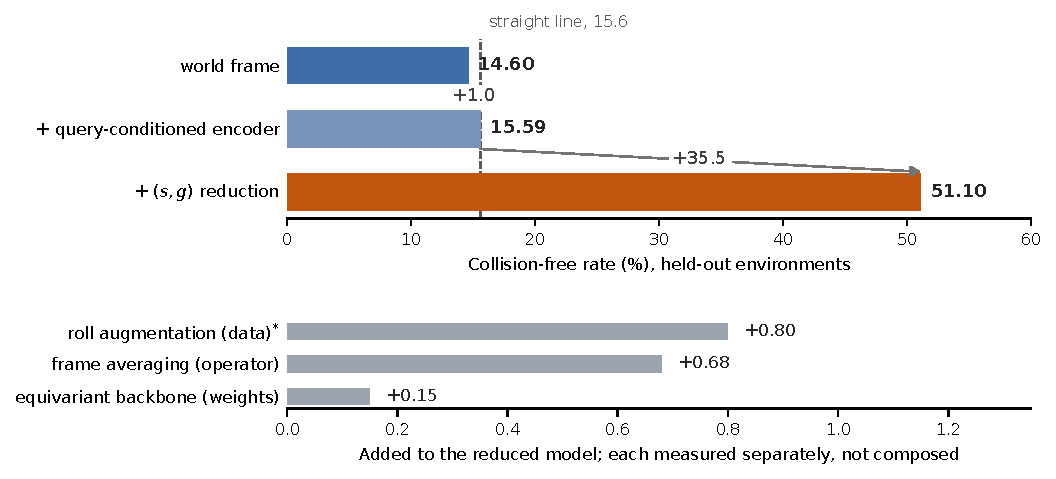
\includegraphics[width=\columnwidth]{fig_cascade.pdf}
\caption{\textbf{Sixty environments, trained to convergence, three seeds}, the
setting used throughout this paper. \emph{Top}: a frame read off the query in
closed form is worth $+35.5$ points, and showing the obstacle encoder the same
query without changing frame is worth $+1.0$. The dashed line is a straight
segment from start to goal on the identical problems, which the world-frame model
does not beat. \emph{Bottom}: the three mechanisms for the one degree of freedom
the frame cannot remove. Each is measured against its own baseline and they are
alternatives rather than a decomposition, so they are not composed here and were
never composed in the experiments.}
\label{fig:teaser}
\end{figure}

% ============================== PAGE 2 (1.0) =========================
\section{Related Work}
% ~250 words. Three clusters, roughly 80 words each: equivariant
% architectures; canonicalisation and frame averaging; generative planners.
\filler{9}

\section{Method}
\subsection{Decomposing the group}
% ~200 words plus the two propositions.
\filler{7}

\begin{proposition}[Lorem ipsum]
\label{prop:one}
Lorem ipsum dolor sit amet, consectetur adipiscing elit, sed do eiusmod tempor
incididunt ut labore et dolore magna aliqua $X' = R_{\hat{x}}(\theta)\,X$.
\end{proposition}

\begin{proposition}[Dolor sit amet]
\label{prop:two}
Lorem ipsum dolor sit amet consectetur adipiscing elit sed do eiusmod tempor
incididunt ut labore.
\end{proposition}
% Two-line proof only. Anything longer goes in an appendix or is cut.
\begin{proof}
Lorem ipsum dolor sit amet consectetur adipiscing elit, sed do eiusmod tempor
incididunt ut labore et dolore magna aliqua ut enim ad minim veniam.
\end{proof}

% ============================== PAGES 3--4 (1.2) =====================
\section{Setup and Calibration}
\subsection{Benchmark and protocol}
% ~180 words. Workspace, obstacle counts, trajectory length, held-out split,
% sample count, integrator budget. Dense and factual; no argument here.
\filler{5}

\begin{table}[t]
\centering
\footnotesize
\setlength{\tabcolsep}{3.5pt}
\begin{tabular}{@{}lrrr@{}}
\toprule
Lorem & Ipsum (\%) & Dolor & s/query \\
\midrule
lorem ipsum          & 00.0 & 0.000 & $<$0.001 \\
dolor sit            & 00.0 & 0.000 & 0.000 \\
amet consectetur     & 00.0 & 0.000 & 0.000 \\
adipiscing elit      & 00.0 & 0.000 & 0.000 \\
sed do eiusmod       & 00.0 & 0.000 & 0.000 \\
\midrule
tempor incididunt    & 00.0 & $-$0.000 & 0.000 \\
ut labore et dolore  & \textbf{00.0} & $-$0.000 & 0.000 \\
\bottomrule
\end{tabular}
\caption{Lorem ipsum dolor sit amet consectetur adipiscing elit sed do eiusmod
tempor incididunt ut labore et dolore magna aliqua}
\label{tab:floors}
\end{table}

\subsection{The floor, and a paired test against it}
% ~200 words. The trivial baseline, the model that does not beat it, and WHY the
% test is paired rather than a comparison of two independently resampled rates.
\filler{7}

% ============================== PAGES 4--5 (1.3) =====================
\section{Results}
\subsection{Scaling}
% ~220 words.
\filler{7}

\begin{figure}[t]
\centering
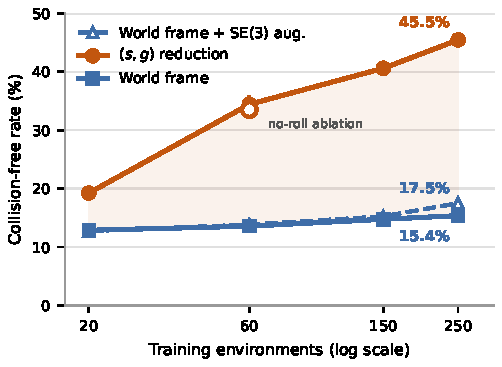
\includegraphics[width=\columnwidth]{fig_scaling_col.pdf}
\caption{Lorem ipsum dolor sit amet consectetur adipiscing elit}
\label{fig:scaling}
\end{figure}

\begin{table}[t]
\centering
\footnotesize
\setlength{\tabcolsep}{3.5pt}
% MERGED mechanism table: one row per mechanism, one column per budget.
\begin{tabular}{@{}l r r >{\raggedright\arraybackslash}p{1.7cm}@{}}
\toprule
Lorem ipsum & A & B & Dolor \\
\midrule
lorem ipsum dolor      & $+00.0$ & $+00.0$ & sit amet \\
\quad consectetur      & $+00.0$ & ---     & adipiscing \\
\quad elit sed         & $+00.0$ & ---     & eiusmod \\
tempor incididunt      & $+0.0$  & ---     & ut labore \\
et dolore magna        & $+0.0$  & $+0.00$ & aliqua \\
ut enim ad minim       & ---     & $+0.00$ & veniam quis \\
\bottomrule
\end{tabular}
\caption{Lorem ipsum dolor sit amet consectetur adipiscing elit sed do eiusmod}
\label{tab:mechanisms}
\end{table}

\begin{figure}[t]
\centering
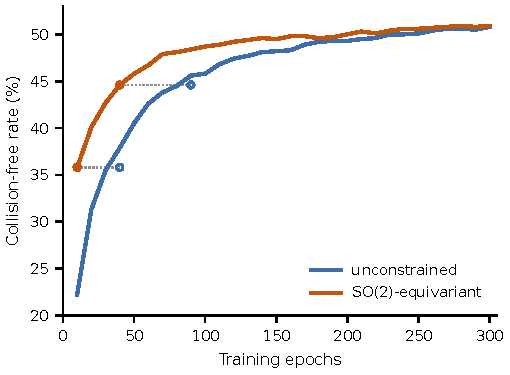
\includegraphics[width=\columnwidth]{fig_convergence.pdf}
\caption{Lorem ipsum dolor sit amet consectetur adipiscing}
\label{fig:conv}
\end{figure}

% ============================== PAGES 5--6 (1.2) =====================
\subsection{Control: a query-conditioned encoder}
% ~250 words. State the deflationary objection in its STRONGEST form first,
% then the model built to test it, then the number.
\filler{9}

\subsection{Control: local geometry, and how it scales}
% ~300 words. The 2x2, the value that survives, the honest ordering, and the
% decay at matched budget.
\filler{9}

\begin{table}[t]
\centering
\footnotesize
\setlength{\tabcolsep}{3.5pt}
\begin{tabular}{@{}lrrr@{}}
\toprule
Lorem ipsum & Dolor & Sit & $\Delta$ \\
\midrule
lorem ipsum       & 00.00 & 00.00 & $+00.0$ \\
dolor sit amet    & 00.00 & 00.00 & $+00.0$ \\
\quad consectetur & 00.00 & \textbf{00.00} & $+00.0$ \\
\midrule
\emph{adipiscing} & $+00.0$ & $+00.0$ & \\
\bottomrule
\end{tabular}
\caption{Lorem ipsum dolor sit amet consectetur adipiscing elit sed do eiusmod
tempor incididunt}
\label{tab:twobytwo}
\end{table}

% ============================== PAGE 6--7 (0.8) ======================
\subsection{Replications}
% ~180 words covering all three at once. One table, three blocks of rows.
\filler{5}

\begin{table}[t]
\centering
\footnotesize
\setlength{\tabcolsep}{3.5pt}
\begin{tabular}{@{}llrrr@{}}
\toprule
Lorem & Ipsum & A & B & $\Delta$ \\
\midrule
dolor   & sit amet     & 00.0 & 00.0 & $+00.0$ \\
        & consectetur  & 00.0 & 00.0 & $+00.0$ \\
\midrule
elit    & sed do       & 00.0 & 00.0 & $+00.0$ \\
        & eiusmod      & 00.0 & 00.0 & $+00.0$ \\
\midrule
tempor  & incididunt   & 00.0 & 00.0 & $+00.0$ \\
        & ut labore    & 00.0 & 00.0 & $+00.0$ \\
\bottomrule
\end{tabular}
\caption{Lorem ipsum dolor sit amet consectetur adipiscing elit}
\label{tab:replications}
\end{table}

\subsection{The residual, and what it bounds}
% A THIRD OF A COLUMN. ~120 words plus the corollary. State the bound, state
% that it does not predict, cite the prior work for the projection property,
% and stop.
\filler{4}

\begin{corollary}[Lorem ipsum]
\label{cor:budget}
Lorem ipsum dolor sit amet consectetur adipiscing elit, sed do eiusmod tempor
incididunt $\|f - \mathcal{A}f\|^2 \le r^2$.
\end{corollary}

% ============================== PAGE 7 (0.8) =========================
\section{Limitations}
% ~200 words. Scope condition first, then seeds, then the single benchmark
% family. Keep the self-corrections: they cost little and buy credibility.
\filler{7}

\section{Conclusion}
% ~120 words. Shorter than feels comfortable.
\filler{4}

% ============================== (0.7) ================================
\section*{Acknowledgements}

The authors thank the IWIN-FINS Laboratory at Shanghai Jiao Tong University for
the computational resources used in this work.

The software implementation was carried out with Claude Code under the first
author's direction. The implementations of the classical planners used to
generate expert trajectories follow the published
algorithms~\cite{kuffner2000rrtconnect,zucker2013chomp,schulman2014trajopt} and
their public reference implementations. The problem formulation, the theoretical
analysis, the experimental design and the text of this paper are the authors'
own. Every reported number is produced by the released code, whose geometric and
equivariance-critical components are verified by property-based tests that run on
untrained networks and include negative controls.

\small
\begin{thebibliography}{99}

\bibitem{albergo2023interpolants}
M.~S. Albergo and E.~Vanden-Eijnden.
\newblock Building normalizing flows with stochastic interpolants.
\newblock In {\em ICLR}, 2023.

\bibitem{bronstein2021gdl}
M.~M. Bronstein, J.~Bruna, T.~Cohen, and P.~Veli\v{c}kovi\'{c}.
\newblock Geometric deep learning: Grids, groups, graphs, geodesics, and gauges.
\newblock {\em arXiv:2104.13478}, 2021.

\bibitem{carvalho2023mpd}
J.~Carvalho, A.~T. Le, M.~Baierl, D.~Koert, and J.~Peters.
\newblock Motion planning diffusion: Learning and planning of robot motions with
  diffusion models.
\newblock In {\em IROS}, 2023.

\bibitem{chi2023dp}
C.~Chi, S.~Feng, Y.~Du, Z.~Xu, E.~Cousineau, B.~Burchfiel, and S.~Song.
\newblock Diffusion policy: Visuomotor policy learning via action diffusion.
\newblock In {\em RSS}, 2023.

\bibitem{cohen2016gcnn}
T.~S. Cohen and M.~Welling.
\newblock Group equivariant convolutional networks.
\newblock In {\em ICML}, 2016.

\bibitem{deng2021vn}
C.~Deng, O.~Litany, Y.~Duan, A.~Poulenard, A.~Tagliasacchi, and L.~Guibas.
\newblock Vector neurons: A general framework for {SO(3)}-equivariant networks.
\newblock In {\em ICCV}, 2021.

\bibitem{elesedy2021strict}
B.~Elesedy and S.~Zaidi.
\newblock Provably strict generalisation benefit for equivariant models.
\newblock In {\em ICML}, 2021.

\bibitem{fishman2022mpinets}
A.~Fishman, A.~Murali, C.~Eppner, B.~Peele, B.~Boots, and D.~Fox.
\newblock Motion policy networks.
\newblock In {\em CoRL}, 2022.

\bibitem{fuchs2020se3t}
F.~B. Fuchs, D.~E. Worrall, V.~Fischer, and M.~Welling.
\newblock {SE(3)}-transformers: 3{D} roto-translation equivariant attention
  networks.
\newblock In {\em NeurIPS}, 2020.

\bibitem{geiger2022e3nn}
M.~Geiger and T.~Smidt.
\newblock e3nn: Euclidean neural networks.
\newblock {\em arXiv:2207.09453}, 2022.

\bibitem{gruver2023lie}
N.~Gruver, M.~Finzi, M.~Goldblum, and A.~G. Wilson.
\newblock The {L}ie derivative for measuring learned equivariance.
\newblock In {\em ICLR}, 2023.

\bibitem{janner2022diffuser}
M.~Janner, Y.~Du, J.~B. Tenenbaum, and S.~Levine.
\newblock Planning with diffusion for flexible behavior synthesis.
\newblock In {\em ICML}, 2022.

\bibitem{kaba2023canon}
S.-O. Kaba, A.~K. Mondal, Y.~Zhang, Y.~Bengio, and S.~Ravanbakhsh.
\newblock Equivariance with learned canonicalization functions.
\newblock In {\em ICML}, 2023.

\bibitem{kuffner2000rrtconnect}
J.~J. Kuffner and S.~M. LaValle.
\newblock {RRT}-connect: An efficient approach to single-query path planning.
\newblock In {\em ICRA}, 2000.

\bibitem{lipman2023fm}
Y.~Lipman, R.~T.~Q. Chen, H.~Ben-Hamu, M.~Nickel, and M.~Le.
\newblock Flow matching for generative modeling.
\newblock In {\em ICLR}, 2023.

\bibitem{liu2023rectified}
X.~Liu, C.~Gong, and Q.~Liu.
\newblock Flow straight and fast: Learning to generate and transfer data with
  rectified flow.
\newblock In {\em ICLR}, 2023.

\bibitem{milnor1978hairy}
J.~Milnor.
\newblock Analytic proofs of the ``hairy ball theorem'' and the {B}rouwer fixed
  point theorem.
\newblock {\em American Mathematical Monthly}, 85(7):521--524, 1978.

\bibitem{oord2016wavenet}
A.~van~den Oord, S.~Dieleman, H.~Zen, K.~Simonyan, O.~Vinyals, A.~Graves,
  N.~Kalchbrenner, A.~Senior, and K.~Kavukcuoglu.
\newblock {W}ave{N}et: A generative model for raw audio.
\newblock {\em arXiv:1609.03499}, 2016.

\bibitem{perez2018film}
E.~Perez, F.~Strub, H.~de~Vries, V.~Dumoulin, and A.~Courville.
\newblock {FiLM}: Visual reasoning with a general conditioning layer.
\newblock In {\em AAAI}, 2018.

\bibitem{puny2022fa}
O.~Puny, M.~Atzmon, H.~Ben-Hamu, I.~Misra, A.~Grover, E.~J. Smith, and
  Y.~Lipman.
\newblock Frame averaging for invariant and equivariant network design.
\newblock In {\em ICLR}, 2022.

\bibitem{qi2017pointnet}
C.~R. Qi, H.~Su, K.~Mo, and L.~J. Guibas.
\newblock {P}oint{N}et: Deep learning on point sets for 3{D} classification and
  segmentation.
\newblock In {\em CVPR}, 2017.

\bibitem{qureshi2019mpnet}
A.~H. Qureshi, A.~Simeonov, M.~J. Bency, and M.~C. Yip.
\newblock Motion planning networks.
\newblock In {\em ICRA}, 2019.

\bibitem{ryu2023edf}
H.~Ryu, H.-i. Lee, J.-H. Lee, and J.~Choi.
\newblock Equivariant descriptor fields: {SE(3)}-equivariant energy-based models
  for end-to-end visual robotic manipulation learning.
\newblock In {\em ICLR}, 2023.

\bibitem{schulman2014trajopt}
J.~Schulman, Y.~Duan, J.~Ho, A.~Lee, I.~Awwal, H.~Bradlow, J.~Pan, S.~Patil,
  K.~Goldberg, and P.~Abbeel.
\newblock Motion planning with sequential convex optimization and convex
  collision checking.
\newblock {\em IJRR}, 33(9):1251--1270, 2014.

\bibitem{simeonov2022ndf}
A.~Simeonov, Y.~Du, A.~Tagliasacchi, J.~B. Tenenbaum, A.~Rodriguez, P.~Agrawal,
  and V.~Sitzmann.
\newblock Neural descriptor fields: {SE(3)}-equivariant object representations
  for manipulation.
\newblock In {\em ICRA}, 2022.

\bibitem{thomas2018tfn}
N.~Thomas, T.~Smidt, S.~Kearnes, L.~Yang, L.~Li, K.~Kohlhoff, and P.~Riley.
\newblock Tensor field networks: Rotation- and translation-equivariant neural
  networks for 3{D} point clouds.
\newblock {\em arXiv:1802.08219}, 2018.

\bibitem{urain2023se3dif}
J.~Urain, N.~Funk, J.~Peters, and G.~Chalvatzaki.
\newblock {SE(3)}-{D}iffusion{F}ields: Learning smooth cost functions for joint
  grasp and motion optimization through diffusion.
\newblock In {\em ICRA}, 2023.

\bibitem{wang2024equidp}
D.~Wang, S.~Hart, D.~Surovik, T.~Kelestemur, H.~Huang, H.~Zhao, M.~Yeatman,
  J.~Wang, R.~Walters, and R.~Platt.
\newblock Equivariant diffusion policy.
\newblock In {\em CoRL}, 2024.

\bibitem{yang2024equibot}
J.~Yang, Z.~Cao, C.~Deng, R.~Antonova, S.~Song, and J.~Bohg.
\newblock {E}qui{B}ot: {SIM(3)}-equivariant diffusion policy for generalizable
  and data efficient learning.
\newblock In {\em CoRL}, 2024.

\bibitem{zucker2013chomp}
M.~Zucker, N.~Ratliff, A.~D. Dragan, M.~Pivtoraiko, M.~Klingensmith, C.~M.
  Dellin, J.~A. Bagnell, and S.~S. Srinivasa.
\newblock {CHOMP}: Covariant Hamiltonian optimization for motion planning.
\newblock {\em IJRR}, 32(9-10):1164--1193, 2013.

\end{thebibliography}

\end{document}
